\section{Threats and Challenges}
A successful benchmark has three criterions to fullfil.
First, it has to be \emph{reproducible} for others to replicate.
Second, the results should be \emph{accurate}, which means each time we rerun the benchmark we are expecting the same results.
Finally, it should \emph{represent} the real world.
In other words, the conclusions brought from the experiment should be valid outside the experimentation as well.
In my case, the real world is the production environment.
Therefore, our experiments should reflect what is happening in the production environments.
In this section, I will deeper dig in each aspect, present what has been done by others and my contributions, and finally I will propose some perspectives, to improve such experiments.

%%%%%%%%% preliminary taughts and section structure 
% The need of reproducibility in our field - software optimization based on empirical studies -

% The importance of Virtualisation for reproducibility \cite{howe_virtual_2012}
% some of the most important parts are
% - fewer constraints on research methods
% - on-demand backups
% - virtual Machines as Publications
% - more Variables captured

\subsection{Reproducibility}
One of the most difficult challenges faced by researchers is the reproducibility of their benchmarks.
Actually, many results fail to be reproduced,\footnote{Trouble at the lab, The Economist, 19 October 2013;  www.economist.com/news/briefing/ 21588057-scientists-think-science-self-correcting- alarming-degree-it-not-trouble.} which led to a \emph{replication crisis}.
As this crisis hit most of the empirical studies, most of the reviews now includes reproducibility as one of the minimal standard for judging scientific merit.\cite{peng2011reproducible}
One of the criterions supporting reproducibility is the publication of the dataset and the algorithms run on the raw data to conclude the results.
There is even some disagreement about what the terms "reproducibility" or "replicability" by themselves mean \cite{goodman2016does}.
According to \cite{echtler2018open}, \emph{replicability} extends \emph{reproducibility} with the ability to collect a new raw dataset comparable to the original one by re-executing the experiment under similar condition, instead of just the ability to get the same results by running the statistical analyses on the original data set.

In the area covered by this PhD thesis, reproducibility might be achieved by ensuring the same execution settings of physical nodes, virtual machines, clusters or cloud environments.
However, when it comes to measuring the energy consumption of a system, applying acknowledged guidelines and carefully repeating the same benchmark can nonetheless lead to different energy footprints not only among homogeneous nodes, but even within a single node.

One major problem that hinders the reproducibility of the empirical benchmarks is the interaction with the external environment, either as concurrency or dependencies.
Therefore, researchers cannot observe the same results, unless they duplicate the same environment.


\subsection{Accuracy}
According to Oxford, \emph{accuracy} means \href{https://www.lexico.com/definition/accuracy}{"technical The degree to which the result of a measurement, calculation, or specification conforms to the correct value or a standard"}.
In ny case, this means the ability to run the benchmark multiple times with a low variation.

Recently, the research community has been investigating typical "crimes" in systems benchmarking and established guidelines for conducting robust and reproducible evaluations~\cite{DBLP:journals/corr/abs-1801-02381}.

In theory, using identical CPU, same memory configuration, similar storage and networking capabilities, should increase the accuracy of physical measurements.
Unfortunately, this is not possible when it comes to measuring the energy consumption of a system.
Applying the benchmarking guidelines and repeating the same experiment with in the same configuration are not sufficient to reproduce the the same energy measurements, not only between identical machines, but even within the same machine.
This difference---also called \emph{energy variation} (EV)---has become a serious threat to the accuracy of experimental evaluations.

%TODO:  rephrase this figure, maybe change it a little bit 
Figure~\ref{fig:motivation} illustrates this variation problem as a violin plot of $20$ executions of the benchmark \emph{Conjugate Gradient} (\textsf{CG}) taken from the \emph{NAS Parallel Benchmarks} (NBP) suite~\cite{Bailey:1991:NPB:125826.125925}, on $4$ nodes of an homogeneous cluster (the cluster \textsf{Dahu} described in Table~\ref{table:g5k}) at 50\,\% workload.
We can observe a large variation of the energy consumption, not only among homogeneous nodes, but also at the scale of a single node, reaching up to $25\,\%$ in this example.

\begin{figure}%[!htb]
    \center{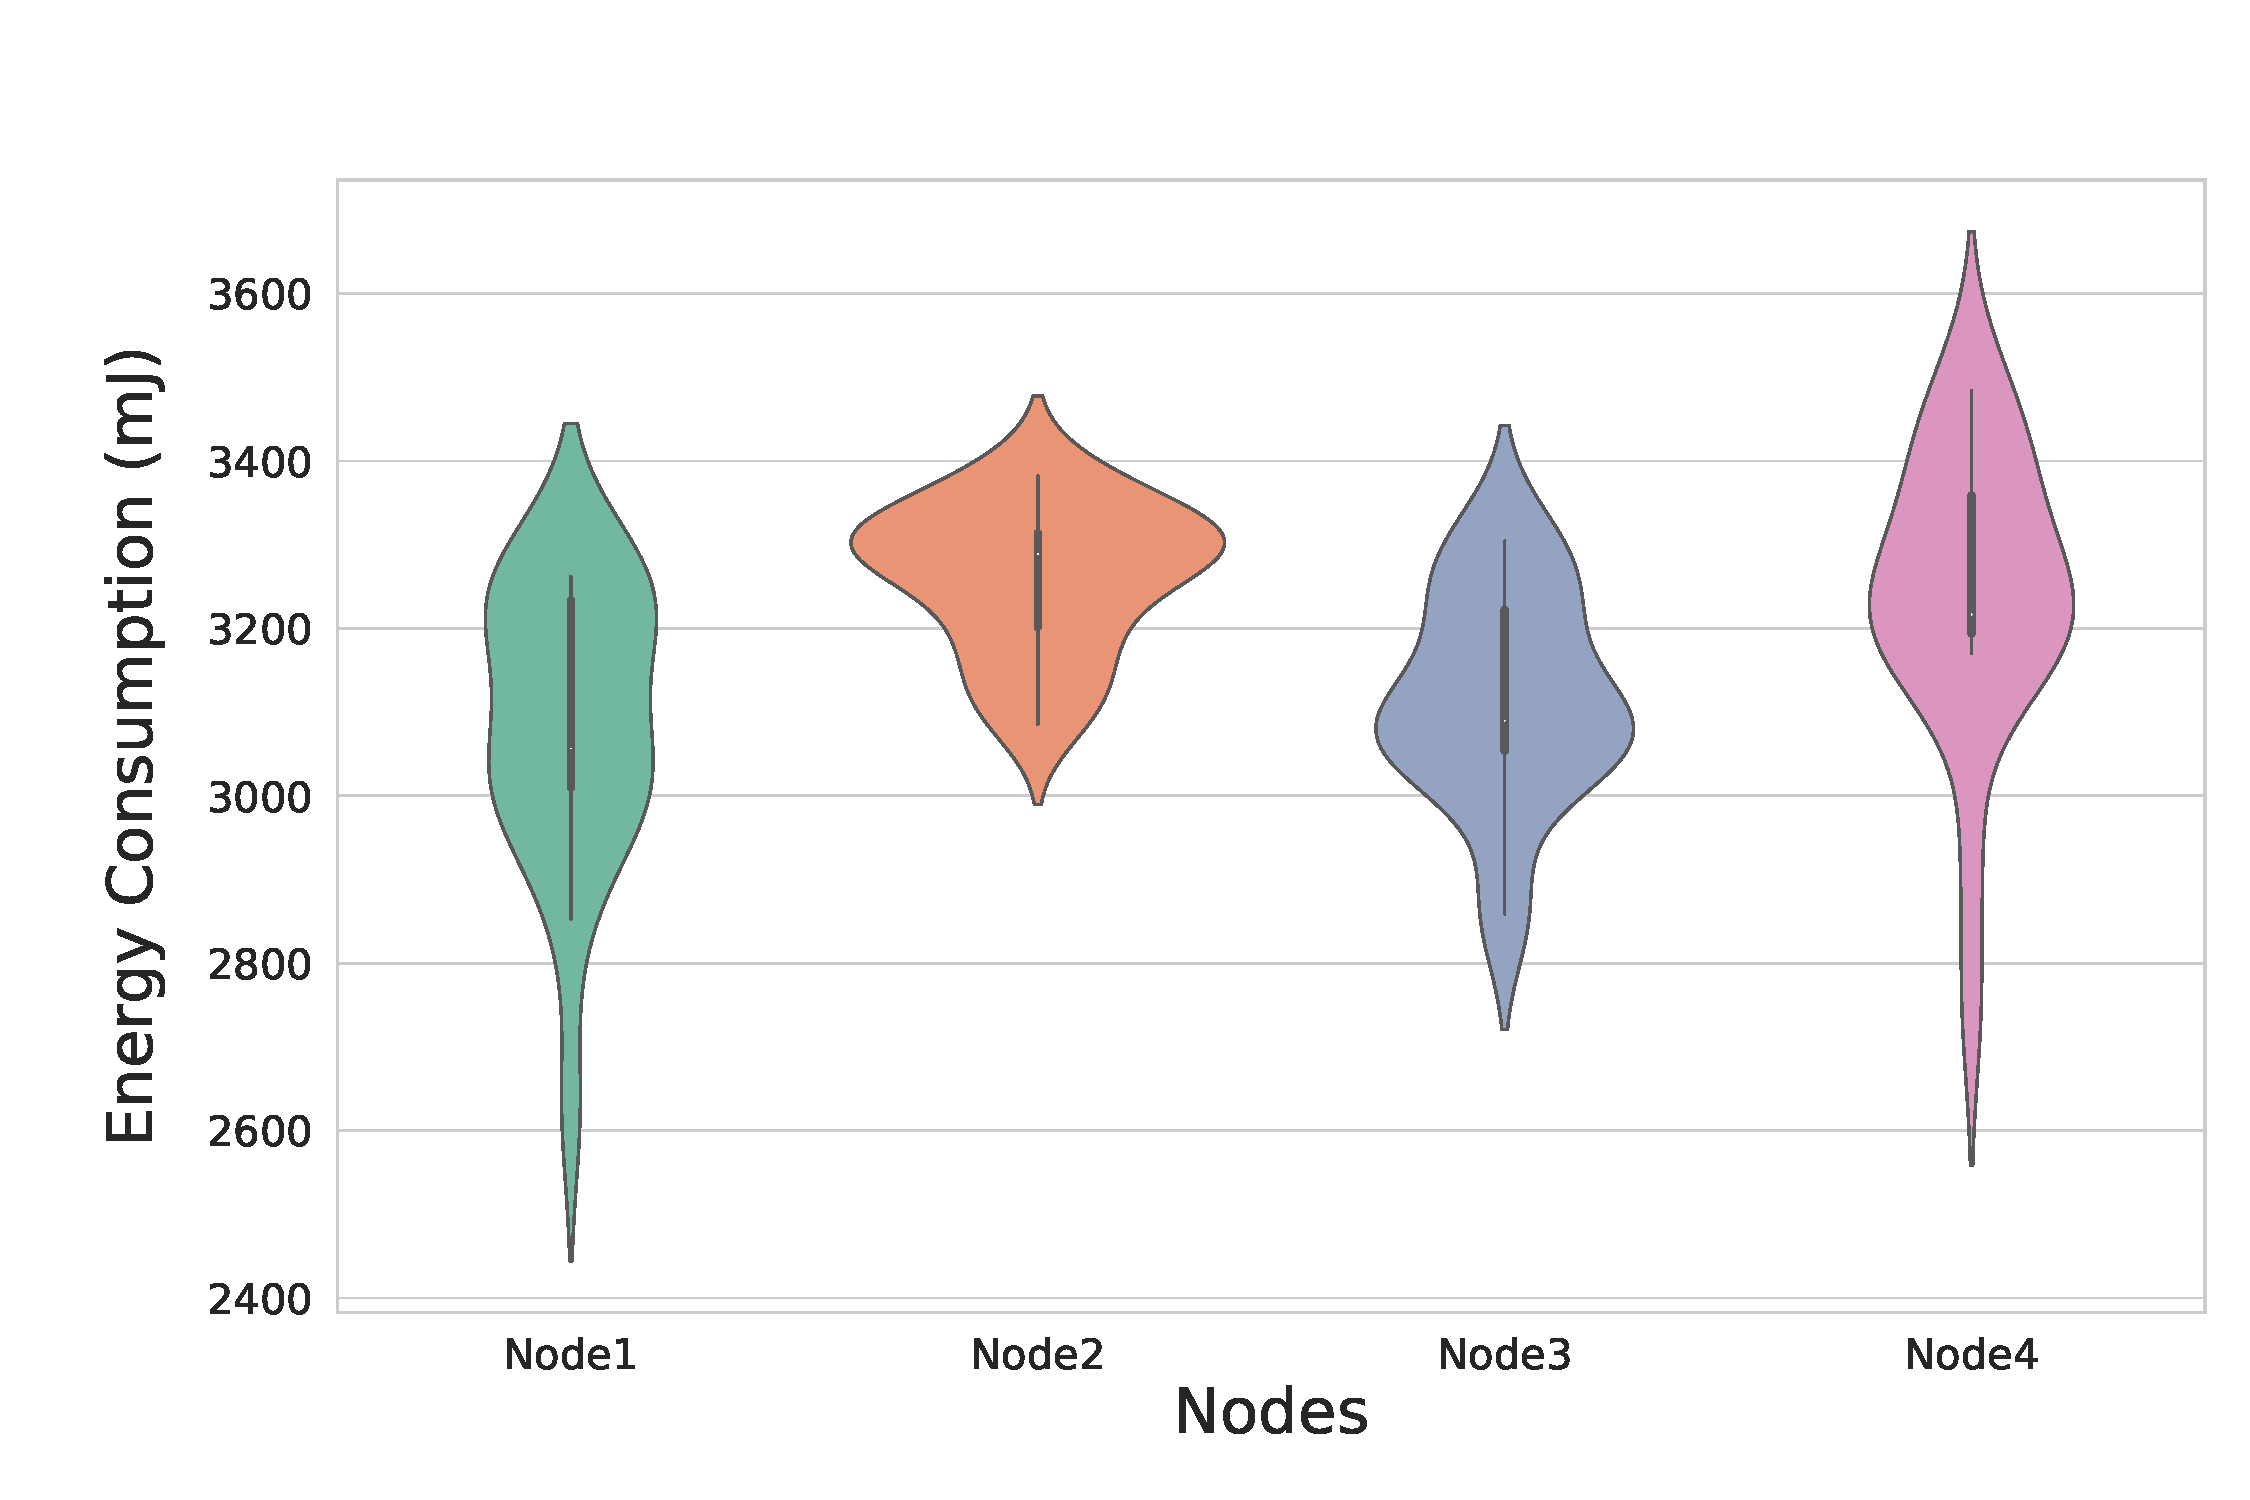
\includegraphics[width=.9\linewidth]{imgs/motivation}}
    \caption{CPU energy variation for the benchmark \textsf{CG}}\label{fig:motivation}
\end{figure}

Some researchers started investigating the hardware impact of the energy variation of power consumption.
As an example, one can cite~\cite{borkar_designing_2005,tschanz_adaptive_2002} who reported that the main cause of the variation of the power consumption between different machines is due to the \textbf{CMOS} manufacturing process of transistors in a chip.
\cite{heinrich_predicting} described this variation as a set of parameters, such as CPU Frequency and the thermal effect.


\subsection{Representativeness}
As obvious as it seems, the reason of executing benchmarks is to validate ideas so we can use them in the real life.
However, this is means that those benchmarks have to represent reality somehow.
Basically, when we aim to benchmark something, we create a mock up version of the situation that we want it to work.
% But, how can we assure that the benchmark is representative? honestly i don't know. and we can't generalize this. but there are some works that have been done for this.
First, we can talk about the benchmarking and their selection, then we will talk about the stress benchmark for some applications, and finally we will bring this representativeness in our case and how can we get closer to the energy consumption behavior of a software between the benchmark environnement and the production one.

As Stephen M. Blackburn~\emph{et~al.} cited in their paper "evaluate collaboratory"~\cite{stephen_evaluate_2012}, one of the major pitfalls of the measurement contexts is the inconsistency, which can be translated here by the fact that the production context is not the same as the benchmarking one.

Another difficult part for practitioners is to generalize the claims they reached beyond the lab conditions.
Are they appropriate?
Are they consistent and are they reproducible?
To answer those questions, the community agreed on some wellknown benchmarks to represent a specific concern of the production world.
One can site as an example the Dacapo and Renaissance benchmark suites for Java applications, or the CLBG benchmark suite for comparing programming languages.
Although they do not cover all the cases, the community agrees on their relevance and representativeness.

In addition to those benchmarks, a new category of benchmarking technique emerged to simulate the worst case of the production environments, inlcuding performance tests, which are benchmarks meant to evaluate the behavior of a software under stress situations.
We can cite as an example the Gatling for web application and stress-ng for hardwares.%ROMAIN: Add citations.
%% YEP I KNOW, THIS IS JUST FOR ME TO READ IT LATER AND GIVE A BETTER CONTEXT
